\documentclass[border=6pt]{standalone}
\usepackage{tikz}
\usetikzlibrary{arrows.meta,positioning,calc,shapes.geometric,fit,backgrounds,patterns,matrix,decorations.pathreplacing}
\begin{document}
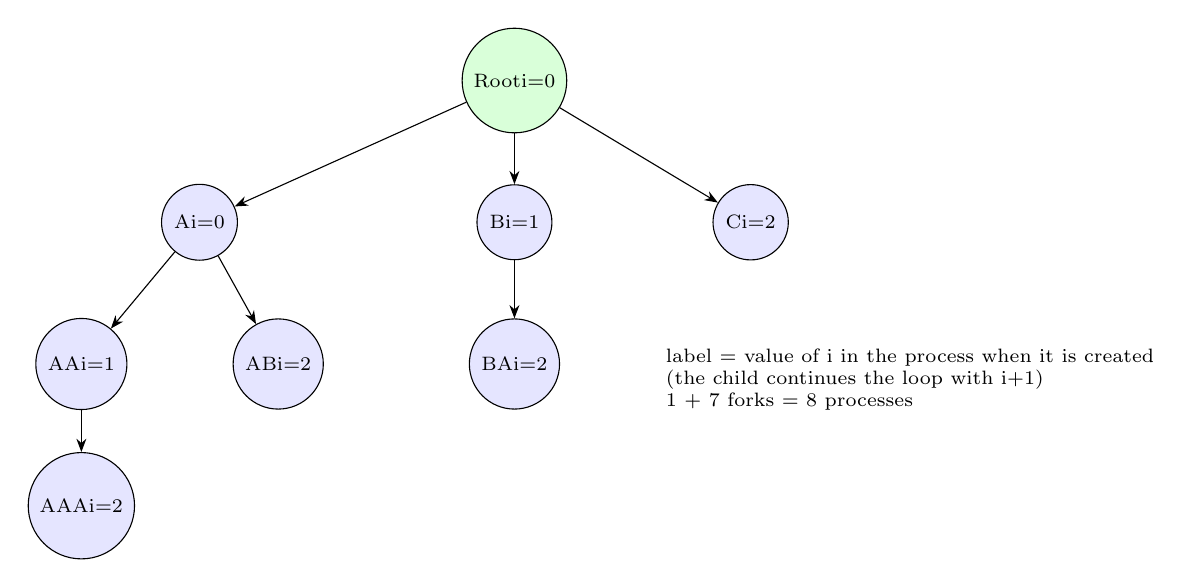
\begin{tikzpicture}[>=Stealth,font=\small]
\tikzstyle{p}=[draw,circle,minimum size=0.8cm,font=\scriptsize,fill=blue!10]
\node[p,fill=green!15] (r) at (0,0) {Root\\ i=0};
\node[p] (a) at (-4,-1.8) {A\\ i=0}; \node[p] (b) at (0,-1.8) {B\\ i=1}; \node[p] (c) at (3,-1.8) {C\\ i=2};
\node[p] (aa) at (-5.5,-3.6) {AA\\ i=1}; \node[p] (ab) at (-3,-3.6) {AB\\ i=2}; \node[p] (ba) at (0,-3.6) {BA\\ i=2};
\node[p] (aaa) at (-5.5,-5.4) {AAA\\ i=2};
\draw[->] (r) -- (a); \draw[->] (r) -- (b); \draw[->] (r) -- (c);
\draw[->] (a) -- (aa); \draw[->] (a) -- (ab); \draw[->] (b) -- (ba); \draw[->] (aa) -- (aaa);
\node[font=\scriptsize,align=left,anchor=west] at (1.8,-3.8) {label = value of i in the process when it is created\\ (the child continues the loop with i+1)\\ 1 + 7 forks = 8 processes};
\end{tikzpicture}
\end{document}
